% Created 2021-06-28 Mon 16:53
% Intended LaTeX compiler: pdflatex
\documentclass[12pt]{article}

%%%% settings when exporting code %%%% 

\usepackage{listings}
\lstdefinestyle{code-small}{
backgroundcolor=\color{white}, % background color for the code block
basicstyle=\ttfamily\small, % font used to display the code
commentstyle=\color[rgb]{0.5,0,0.5}, % color used to display comments in the code
keywordstyle=\color{black}, % color used to highlight certain words in the code
numberstyle=\ttfamily\tiny\color{gray}, % color used to display the line numbers
rulecolor=\color{black}, % color of the frame
stringstyle=\color[rgb]{0,.5,0},  % color used to display strings in the code
breakatwhitespace=false, % sets if automatic breaks should only happen at whitespace
breaklines=true, % sets automatic line breaking
columns=fullflexible,
frame=single, % adds a frame around the code (non,leftline,topline,bottomline,lines,single,shadowbox)
keepspaces=true, % % keeps spaces in text, useful for keeping indentation of code
literate={~}{$\sim$}{1}, % symbol properly display via latex
numbers=none, % where to put the line-numbers; possible values are (none, left, right)
numbersep=10pt, % how far the line-numbers are from the code
showspaces=false,
showstringspaces=false,
stepnumber=1, % the step between two line-numbers. If it's 1, each line will be numbered
tabsize=1,
xleftmargin=0cm,
emph={anova,apply,class,coef,colnames,colNames,colSums,dim,dcast,for,ggplot,head,if,ifelse,is.na,lapply,list.files,library,logLik,melt,plot,require,rowSums,sapply,setcolorder,setkey,str,summary,tapply},
aboveskip = \medskipamount, % define the space above displayed listings.
belowskip = \medskipamount, % define the space above displayed listings.
lineskip = 0pt} % specifies additional space between lines in listings
\lstset{style=code-small}
%%%% packages %%%%%

\usepackage[utf8]{inputenc}
\usepackage[T1]{fontenc}
\usepackage{lmodern}
\usepackage{textcomp}
\usepackage{color}
\usepackage{graphicx}
\usepackage{grffile}
\usepackage{wrapfig}
\usepackage{rotating}
\usepackage{longtable}
\usepackage{multirow}
\usepackage{multicol}
\usepackage{changes}
\usepackage{pdflscape}
\usepackage{geometry}
\usepackage[normalem]{ulem}
\usepackage{amssymb}
\usepackage{amsmath}
\usepackage{amsfonts}
\usepackage{dsfont}
\usepackage{array}
\usepackage{ifthen}
\usepackage{hyperref}
\usepackage{natbib}
%
%%%% specifications %%%%
%
\usepackage{ifthen}
\usepackage{xifthen}
\usepackage{xargs}
\usepackage{xspace}
\newcommand\Rlogo{\textbf{\textsf{R}}\xspace} %
\usepackage{xr} %% read the .aux of the external file
\externaldocument[SM-]{SM-article-Ustatistic-nuisance}
\newcommand\Xobs{\tilde{X}}
\newcommand\Yobs{\tilde{Y}}
\newcommand\xobs{\tilde{x}}
\newcommand\yobs{\tilde{y}}
\newcommand\Xcens{\delta}
\newcommand\Ycens{\varepsilon}
\newcommand\Xcount{N_{X}}
\newcommand\Ycount{N_{Y}}
\newcommand\Xrisk{R_{X}}
\newcommand\Yrisk{R_{Y}}
\newcommand\DeltaHat{\hat{\Delta}}
\newcommand\U{U}
\newcommand\UHat{\hat{U}}
\newcommand\Ufav{U^{+}}
\newcommand\Udefav{U^{-}}
\newcommand\UfavHat{\UHat^{+}}
\newcommand\UdefavHat{\UHat^{-}}
\newcommand\s{s}
\newcommand\sfav{s^{+}}
\newcommand\sdefav{s^{-}}
\newcommand\IF{h}
\newcommand\IFfav{h^{+}}
\newcommand\IFdefav{h^{-}}
\newcommand\IFfavHat{\hat{h}^{+}}
\newcommand\IFdefavHat{\hat{h}^{-}}
\newcommand\sigmaApprox{\tilde{\sigma}}
\newcommand\sigmaHat{\hat{\sigma}}
\newcommand\param{\eta}
\newcommand\Vparam{\boldsymbol{\eta}}
\newcommand\VparamHat{\hat{\Vparam}}
\newcommand\Xsurv{S_{X}}
\newcommand\Ysurv{S_{Y}}
\newcommand\XsurvHat{\hat{S}_{X}}
\newcommand\YsurvHat{\hat{S}_{Y}}
\newcommand\Xhazard{\lambda_{X}}
\newcommand\Yhazard{\lambda_{Y}}
\newcommand\XhazardHat{\hat{\lambda}_{X}}
\newcommand\YhazardHat{\hat{\lambda}_{Y}}
\RequirePackage{fancyvrb} % fancybox
\DefineVerbatimEnvironment{verbatim}{Verbatim}{fontsize=\small,formatcom = {\color[rgb]{0.5,0,0}}}
\RequirePackage{colortbl} % arrayrulecolor to mix colors
\RequirePackage{setspace} % to modify the space between lines - incompatible with footnote in beamer
\renewcommand{\baselinestretch}{1}
\geometry{top=1cm}
\hypersetup{
citecolor=[rgb]{0,0.5,0},
urlcolor=[rgb]{0,0,0.5},
linkcolor=[rgb]{0,0,0.5},
}
\usepackage[framemethod=tikz]{mdframed}
\usetikzlibrary{shadows}
\newmdenv[shadow=true,shadowcolor=black!100,shadowsize=10pt,font=\sffamily,leftmargin=5pt,rightmargin=5pt]{shadedbox}
\RequirePackage{epstopdf} % to be able to convert .eps to .pdf image files
\RequirePackage{capt-of} %
\RequirePackage{caption} % newlines in graphics
\RequirePackage{amsmath}
\RequirePackage{algorithm}
\RequirePackage[noend]{algpseudocode}
\RequirePackage{dsfont}
\RequirePackage{amsmath,stmaryrd,graphicx}
\RequirePackage{prodint} % product integral symbol (\PRODI)
\newcommand\defOperator[7]{%
\ifthenelse{\isempty{#2}}{
\ifthenelse{\isempty{#1}}{#7{#3}#4}{#7{#3}#4 \left#5 #1 \right#6}
}{
\ifthenelse{\isempty{#1}}{#7{#3}#4_{#2}}{#7{#3}#4_{#1}\left#5 #2 \right#6}
}
}
\newcommand\defUOperator[5]{%
\ifthenelse{\isempty{#1}}{
#5\left#3 #2 \right#4
}{
\ifthenelse{\isempty{#2}}{\underset{#1}{\operatornamewithlimits{#5}}}{
\underset{#1}{\operatornamewithlimits{#5}}\left#3 #2 \right#4}
}
}
\newcommand{\defBoldVar}[2]{
\ifthenelse{\equal{#2}{T}}{\boldsymbol{#1}}{\mathbf{#1}}
}
\newcommandx\Cov[2][1=,2=]{\defOperator{#1}{#2}{C}{ov}{\lbrack}{\rbrack}{\mathbb}}
\newcommandx\Esp[2][1=,2=]{\defOperator{#1}{#2}{E}{}{\lbrack}{\rbrack}{\mathbb}}
\newcommandx\Prob[2][1=,2=]{\defOperator{#1}{#2}{P}{}{\lbrack}{\rbrack}{\mathbb}}
\newcommandx\Qrob[2][1=,2=]{\defOperator{#1}{#2}{Q}{}{\lbrack}{\rbrack}{\mathbb}}
\newcommandx\Var[2][1=,2=]{\defOperator{#1}{#2}{V}{ar}{\lbrack}{\rbrack}{\mathbb}}
\newcommandx\Binom[2][1=,2=]{\defOperator{#1}{#2}{B}{}{(}{)}{\mathcal}}
\newcommandx\Gaus[2][1=,2=]{\defOperator{#1}{#2}{N}{}{(}{)}{\mathcal}}
\newcommandx\Wishart[2][1=,2=]{\defOperator{#1}{#2}{W}{ishart}{(}{)}{\mathcal}}
\newcommandx\Likelihood[2][1=,2=]{\defOperator{#1}{#2}{L}{}{(}{)}{\mathcal}}
\newcommandx\Information[2][1=,2=]{\defOperator{#1}{#2}{I}{}{(}{)}{\mathcal}}
\newcommandx\Score[2][1=,2=]{\defOperator{#1}{#2}{S}{}{(}{)}{\mathcal}}
\newcommandx\Hessian[2][1=,2=]{\defOperator{#1}{#2}{H}{}{(}{)}{\mathcal}}
\usepackage{prodint} % product integral symbol (\PRODI)
\newcommandx\Vois[2][1=,2=]{\defOperator{#1}{#2}{V}{}{(}{)}{\mathcal}}
\newcommandx\Ind[1][1=]{\defOperator{}{#1}{1}{}{(}{)}{\mathds}}
\newcommandx\Max[2][1=,2=]{\defUOperator{#1}{#2}{(}{)}{min}}
\newcommandx\Min[2][1=,2=]{\defUOperator{#1}{#2}{(}{)}{max}}
\newcommandx\argMax[2][1=,2=]{\defUOperator{#1}{#2}{(}{)}{argmax}}
\newcommandx\argMin[2][1=,2=]{\defUOperator{#1}{#2}{(}{)}{argmin}}
\newcommandx\cvD[2][1=D,2=n \rightarrow \infty]{\xrightarrow[#2]{#1}}
\newcommandx\Hypothesis[2][1=,2=]{
\ifthenelse{\isempty{#1}}{
\mathcal{H}
}{
\ifthenelse{\isempty{#2}}{
\mathcal{H}_{#1}
}{
\mathcal{H}^{(#2)}_{#1}
}
}
}
\newcommandx\dpartial[4][1=,2=,3=,4=\partial]{
\ifthenelse{\isempty{#3}}{
\frac{#4 #1}{#4 #2}
}{
\left.\frac{#4 #1}{#4 #2}p\right\rvert_{#3}
}
}
\newcommandx\dTpartial[3][1=,2=,3=]{\dpartial[#1][#2][#3][d]}
\newcommandx\ddpartial[3][1=,2=,3=]{
\ifthenelse{\isempty{#3}}{
\frac{\partial^{2} #1}{\partial #2^2}
}{
\frac{\partial^2 #1}{\partial #2\partial #3}
}
}
\newcommand\Real{\mathbb{R}}
\newcommand\Rational{\mathbb{Q}}
\newcommand\Natural{\mathbb{N}}
\newcommand\trans[1]{{#1}^\intercal}%\newcommand\trans[1]{{\vphantom{#1}}^\top{#1}}
\newcommand{\independent}{\mathrel{\text{\scalebox{1.5}{$\perp\mkern-10mu\perp$}}}}
\newcommand\half{\frac{1}{2}}
\newcommand\normMax[1]{\left|\left|#1\right|\right|_{max}}
\newcommand\normTwo[1]{\left|\left|#1\right|\right|_{2}}
\date{}
\title{Simulation study: "Leveraging multimodal data to predict outcomes of antidepressant treatment"}
\hypersetup{
 colorlinks=true,
 pdfauthor={},
 pdftitle={Simulation study: "Leveraging multimodal data to predict outcomes of antidepressant treatment"},
 pdfkeywords={},
 pdfsubject={},
 pdfcreator={Emacs 26.3 (Org mode 9.4.6)},
 pdflang={English}
 }
\begin{document}

\maketitle
\lstset{language=r,label= ,caption= ,captionpos=b,numbers=none}
\begin{lstlisting}
path <- "~/Documents/GitHub/article-predictionNP1BD3/"
setwd(path)
source("./FCT/simData.R")
\end{lstlisting}

\section{Introduction}
\label{sec:org9a1599e}

We proposed a three step strategy to build and assess predictive
models for antidepressant treatment response:
\begin{itemize}
\item \textbf{step 1}: a logistic regression with linear effects and no interest
on a subset of 10 biomarkers
\item \textbf{step 2}: a random forest approach on a subset of 10
biomarkers. Variable importance of each biomarker will be assessed
and a more complex logistic regression (with non-linear effects and
interaction) will be built using only important biomarkers.
\item \textbf{step 3}: SuperLearner will be train on a large set of biomarkers.
\end{itemize}

5-fold cross validation will be used to assess the predictive
performances in term of AUC, brier score, and calibration.

\bigskip

However, there are some difficulties:

\begin{itemize}
\item What is the power of the random forest test vs. logistic? \newline Of
variable importance to detect useful biomarkers? \newline Of the complex
logistic regression to identify complex patterns?

\item there are several way to assess variable importance in random
forest, e.g. \texttt{impurity} based on the Gini index (function
\texttt{importance\_pvalues} in ranger) or the method developped by
\cite{konukoglu2014approximate} (implemented in the R package
forestControl).

\item is the 5-fold cross validation a good way to estimate predictive
performances (bias, variance)\footnote{Martin N. asked something similar
at the Brain Drug annual meeting}? Many other approaches exists so
it would be nice to show that this one leads to reasonable
results\footnote{We could use repeated 10-fold CV where is fold has the same prevalence}.

\item how to choose the hyperparameters of the machine learning approach?
E.g. in random forest we need to choose:
\begin{enumerate}
\item a number of trees (argument \texttt{num.trees} in ranger, by default 500)
\item a number of features considered for splitting a node (argument \texttt{mtry} in ranger, by default square root of the number of predictors)
\item minimal number of data points to split a node (argument \texttt{min.node.size} in ranger, by default 1),
\item maximum tree depth (argument \texttt{max.depth} in ranger, by default unlimited),
\item objective function (argument \texttt{splitrule} in ranger, by default \texttt{"gini"})
\item sampling of the observations (argument \texttt{replace} in ranger, by default \texttt{TRUE})
\end{enumerate}
For superLearner we need to choose:
\begin{enumerate}
\item the library of learner we want to consider (argument
\texttt{SL.library} in SuperLearner).
\item how do we want to combine the learners? Take the best or
combine the prediction of each learner in the best way
possible.
\item plus the hyperparameters corresponding to each learner.
\end{enumerate}
\end{itemize}



\section{Objectives}
\label{sec:org1970248}

Assess the validity of the predictive approach:
\begin{itemize}
\item in term of type 1 error control, i.e. conclude that there a predictive
value when in fact there is none at most \(\alpha\)\% of the time.
\item in term of type 2 error control, i.e. conclude that we cannot identify a predictive
value when in fact there is one at most \(\beta\)\% of the time.
\end{itemize}

\bigskip

Estimate the hyperparameters of the machine learning
approaches. \newline From the existing litterature on Random Forests,
the main parameter to tune is \texttt{mtry}
\cite{probst2019hyperparameters}. Other parameters such as \texttt{num.tree}
can be set to arbitrary large value that is computationnally feasible
\citep{probst2017tune}.  \newline The super learner library should at
least contain Random Forests and elastic-net regularized logistic
regression.

\section{Generative model}
\label{sec:org0603173}

To perform the simulation study, we first start by defining a number
of scenario that should ressemble real data. As there are many parameters we can vary, we will fix:
\begin{itemize}
\item the sample size to \(n=80\).
\item the number of predictors to \(p=10\) and the number of useful
predictors 2 (unless when we are under the null where it is 0).
\item the marginal distribution of each predictor to a multivariate normal
distribution with mean 0 and variance 1. \textcolor{red}{Can
  be changed to better reflect real data!}
\end{itemize}
We will vary:
\begin{itemize}
\item the strenght of the predictors (strong, weak, or null)
\item the type of interaction between the predictors considering 3
scenarios: either no interaction, or normal values vs. abnormal
values, or no main effect and only an interaction.
\item the correlation between the predictors. The predictors will be
divided in two groups and the within group correlation will be
vary. Each group contain a single useful predictor.
\end{itemize}

Visually this can is summarized in \autoref{fig:sim-scenario} and  \autoref{fig:sim-correlation}.
\begin{figure}[htbp]
\centering
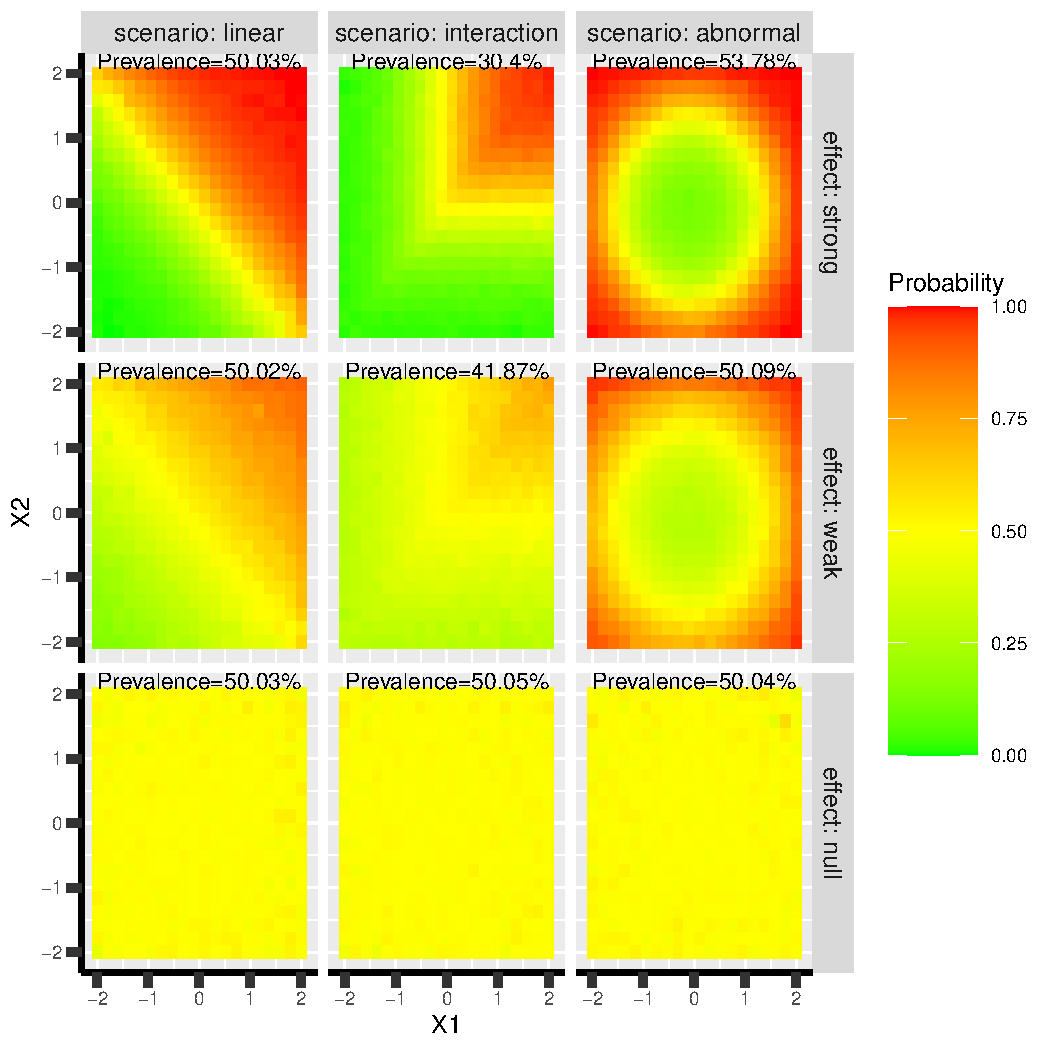
\includegraphics[width=1\textwidth]{./Figures/fig-scenario.pdf}
\caption{\label{fig:sim-scenario}Probability of treatment response as a function of the useful biomarkers in each scenario.}
\end{figure}

\begin{figure}[htbp]
\centering
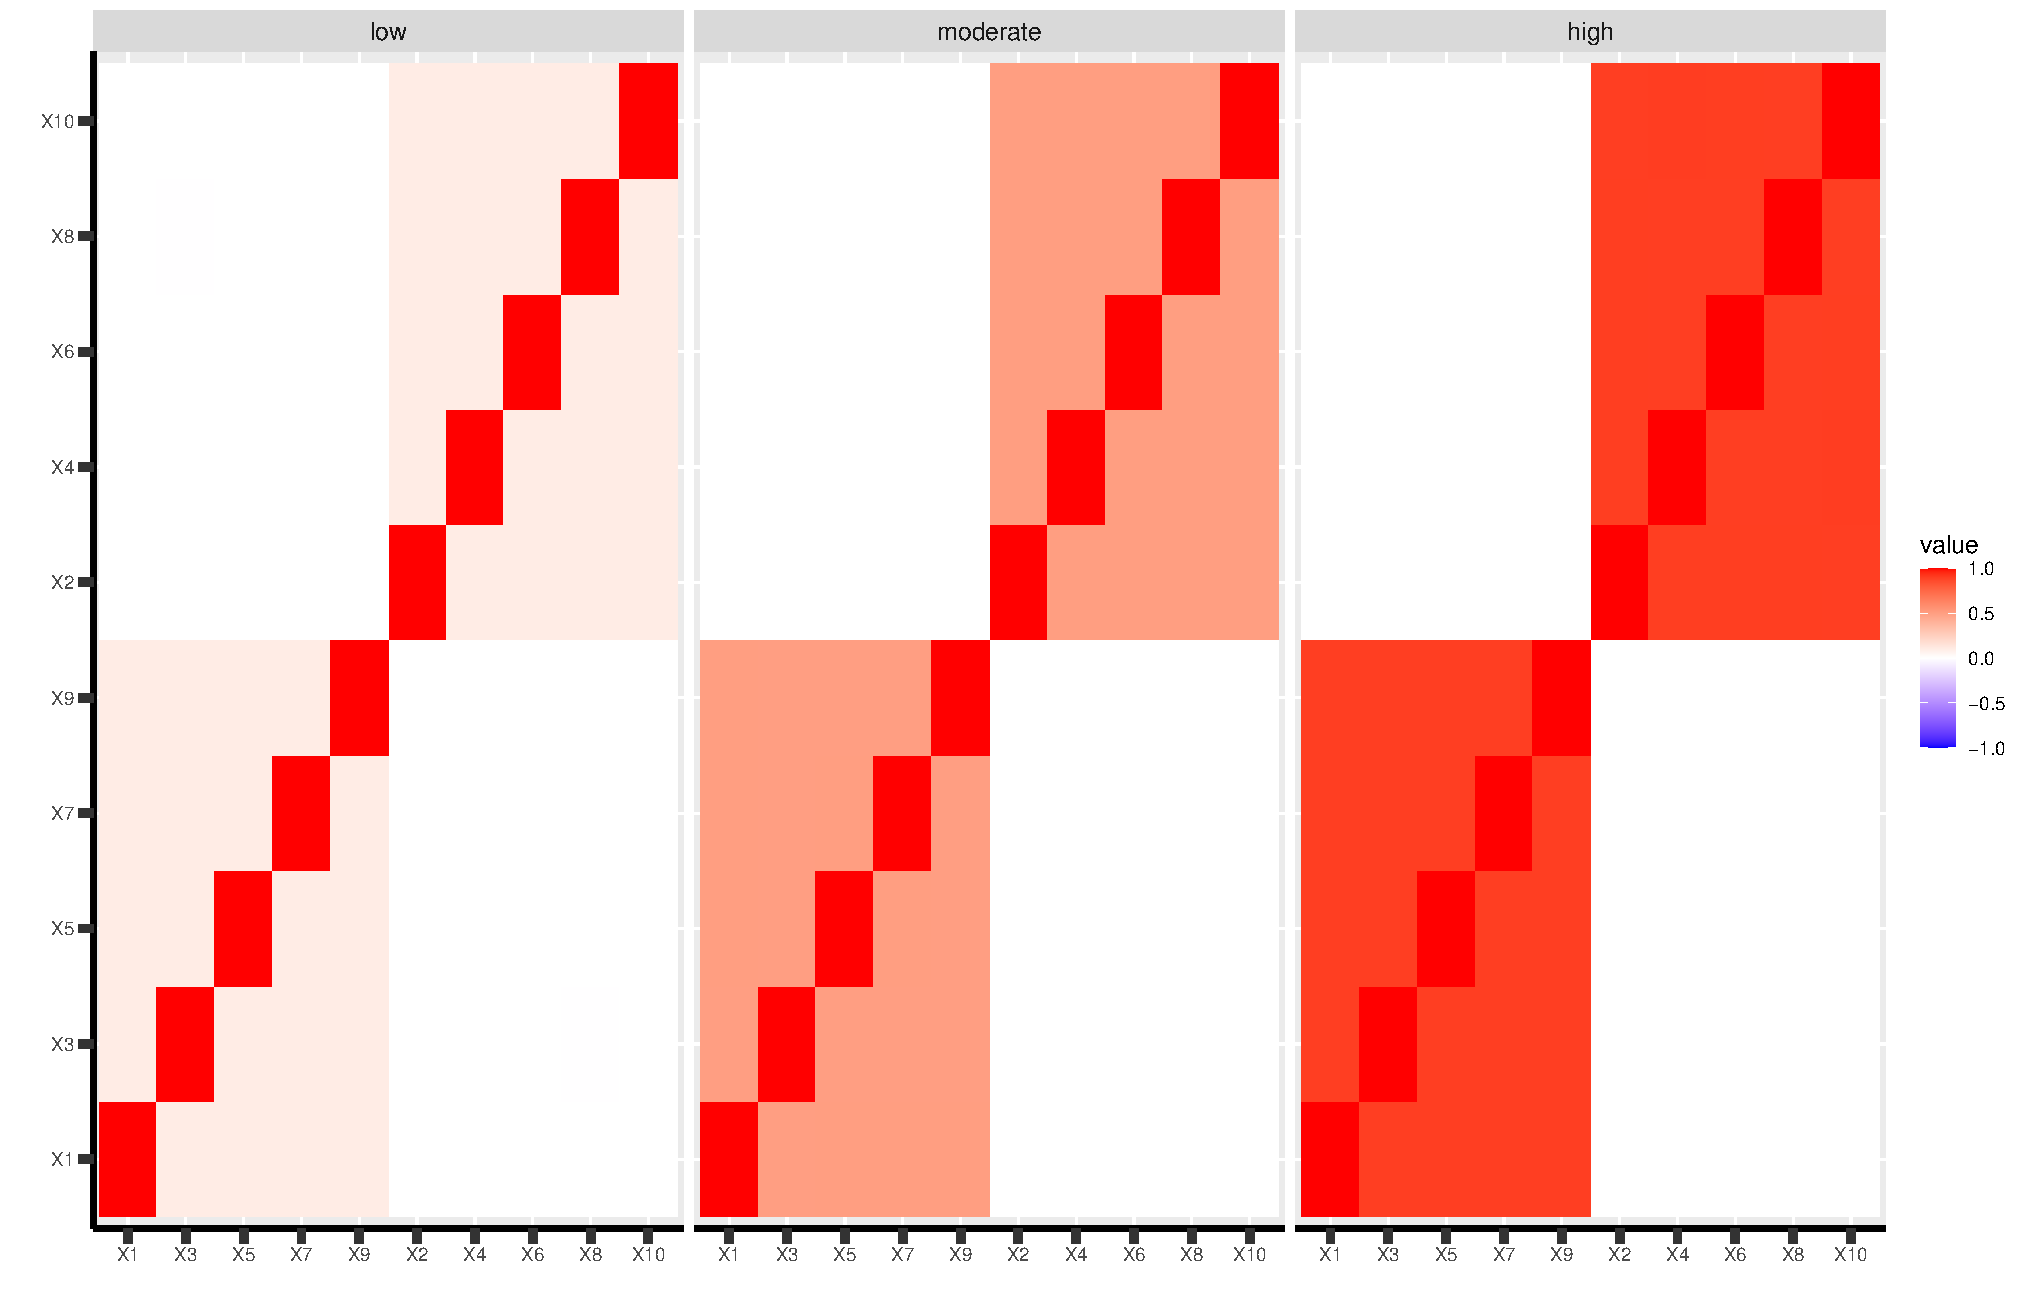
\includegraphics[width=1\textwidth]{./Figures/fig-correlation.pdf}
\caption{\label{fig:sim-correlation}Correlation structure of the predictors.}
\end{figure}


\section{References}
\label{sec:orgfb22c1d}
\begingroup
\renewcommand{\section}[2]{}
\bibliographystyle{unsrt}
\bibliography{bibliography}

\endgroup

\section{Setting}
\label{sec:org1120dc9}
\end{document}